\subsection{\textsf{FSM}: A \DSL for Finite-State Machines}
\label{sec:Examples:FSM}

Finite State Machines (FSM) represent a common \DSL for capturing state-based 
behaviour of various biological, but also computational domains (e.g. Chomsky's 
Regular Grammars, among others). We consider
FSMs that are simplified in various ways: in particular, we target a
\emph{word-acceptance} semantics, where transitions do not contain guards and 
triggers are reduced to their simplest expression, namely simple strings.

\subsubsection{Specification}
\label{sec:Examples:FSM:Specification}

\begin{figure}[t]%
   \centering
   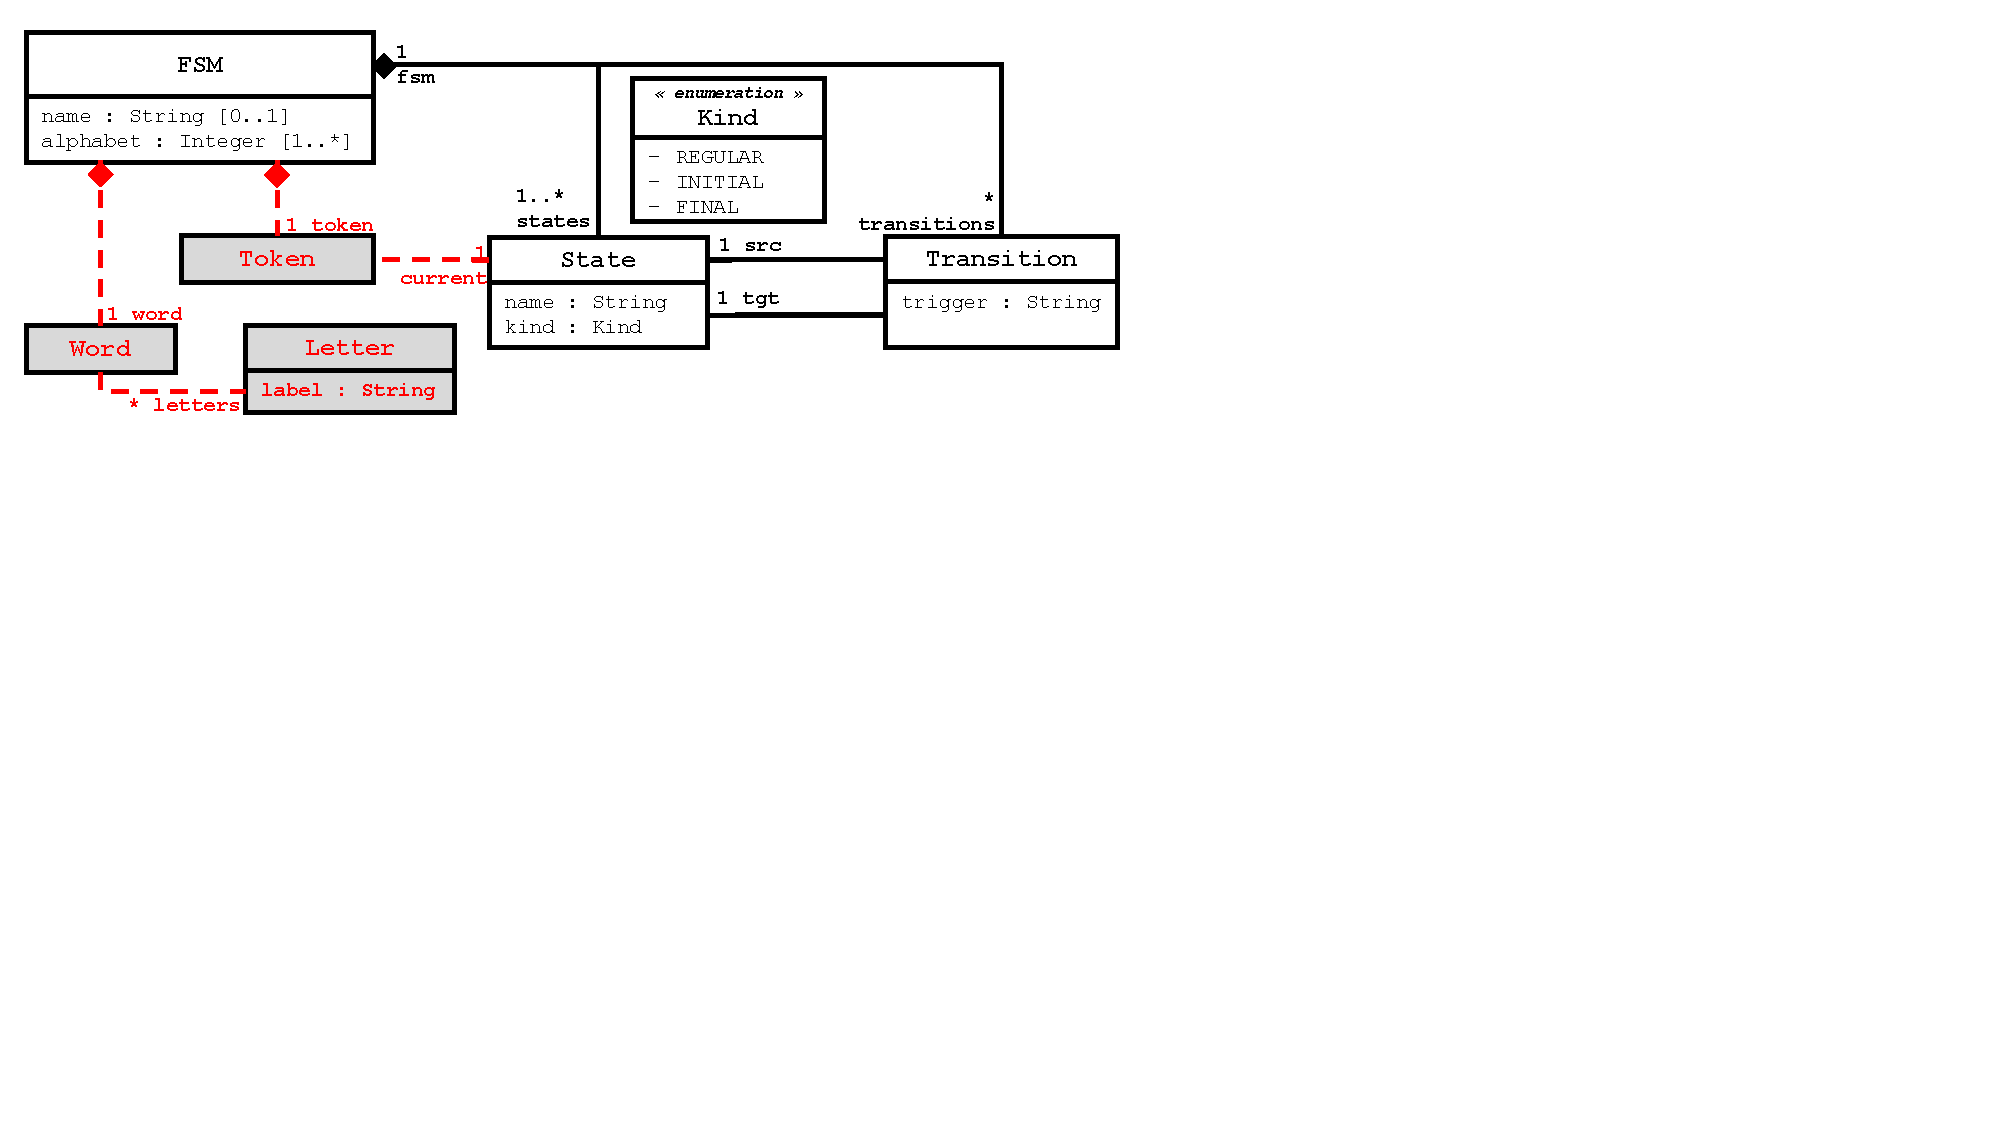
\includegraphics[width=\columnwidth, clip, trim=0.3cm 12cm 14.5cm 0.3cm]{FSM_MM}%
   \caption{A metamodel for Finite State Machines.}%
   \label{fig:FSM_MM}%
   \Description[A Simple Metamodel for Finite State Machines]{A simple metamodel for Finite State Machines}
\end{figure}

\begin{figure}[t]%
   \centering
   \begin{subfigure}[b]{0.45\columnwidth}
      \centering
      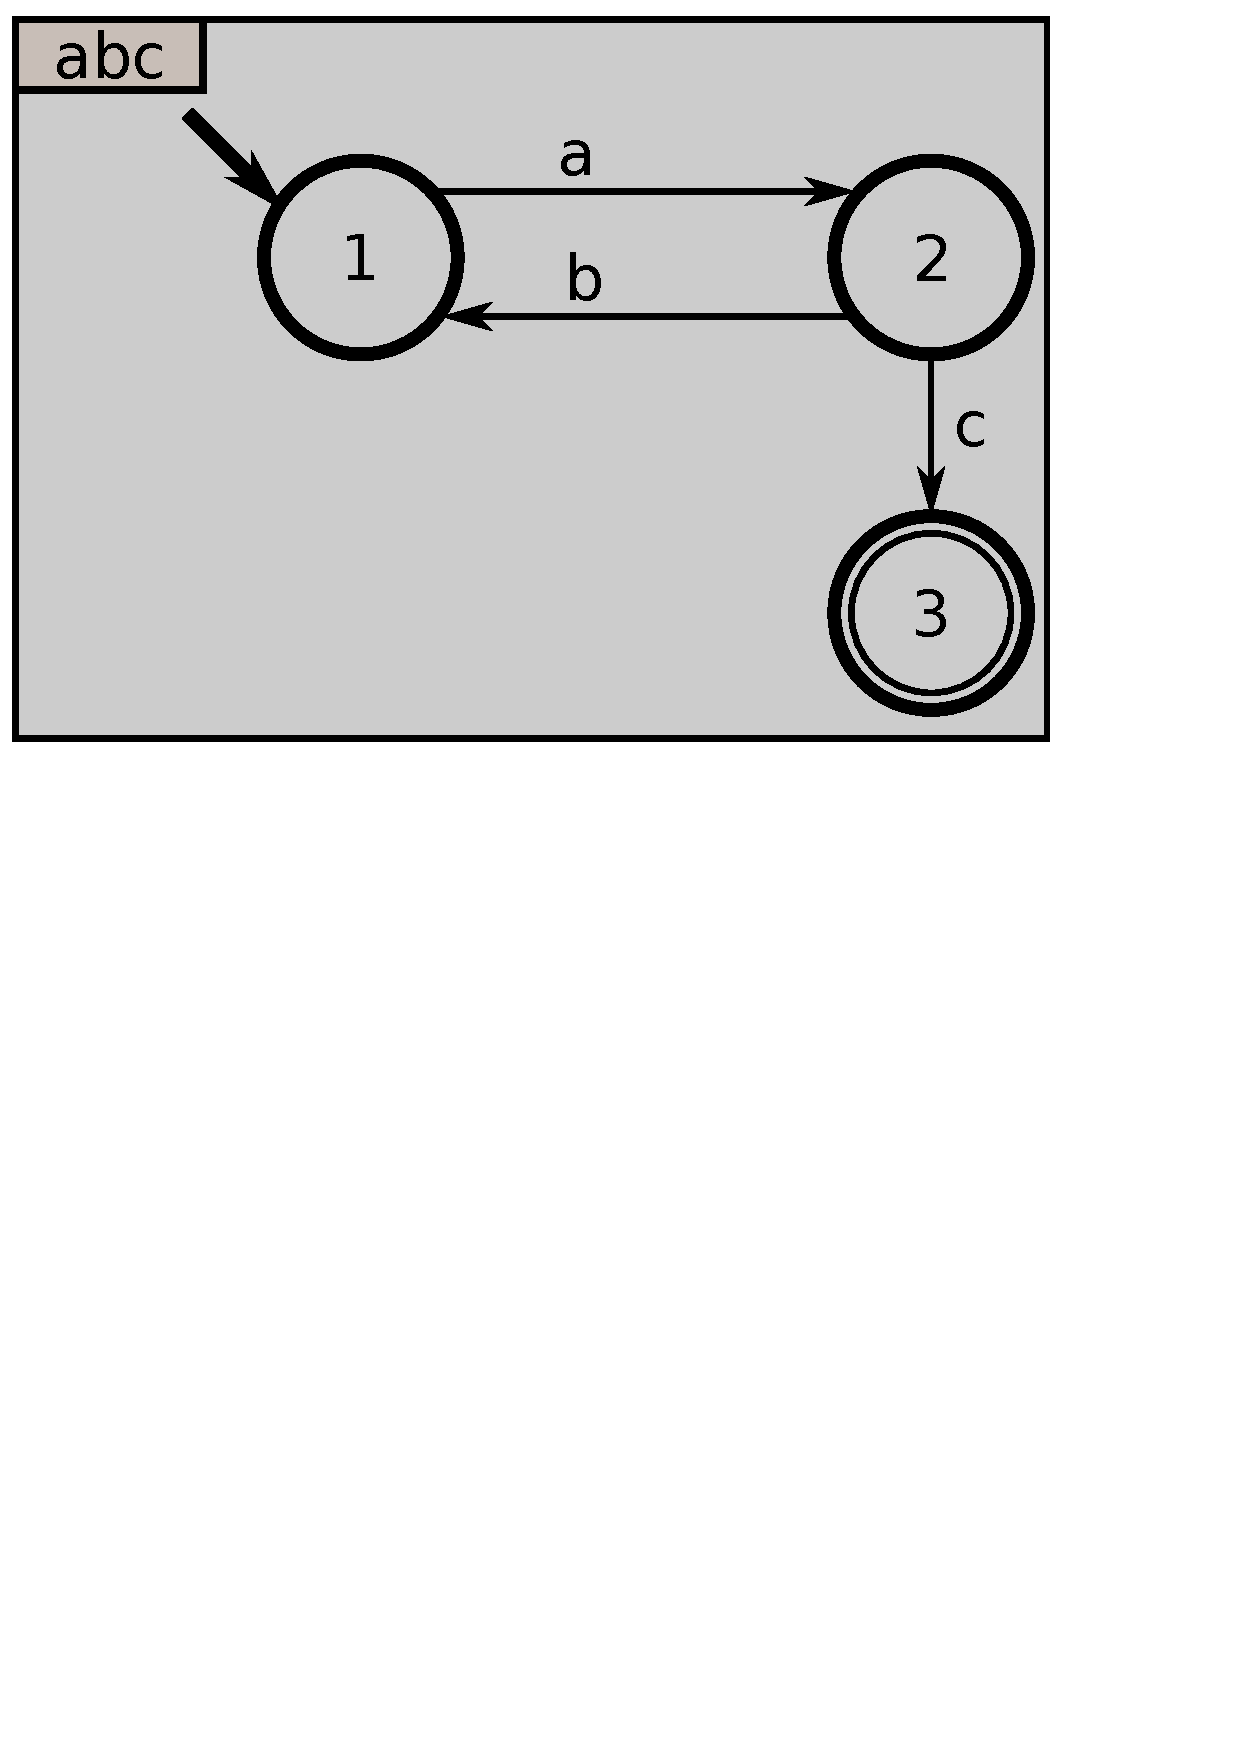
\includegraphics[width=\columnwidth, clip, trim=0cm 17cm 3cm 0cm]{FSM_M.pdf}%
   \end{subfigure}
   \hfill
   \begin{subfigure}[b]{0.45\columnwidth}
      \centering
      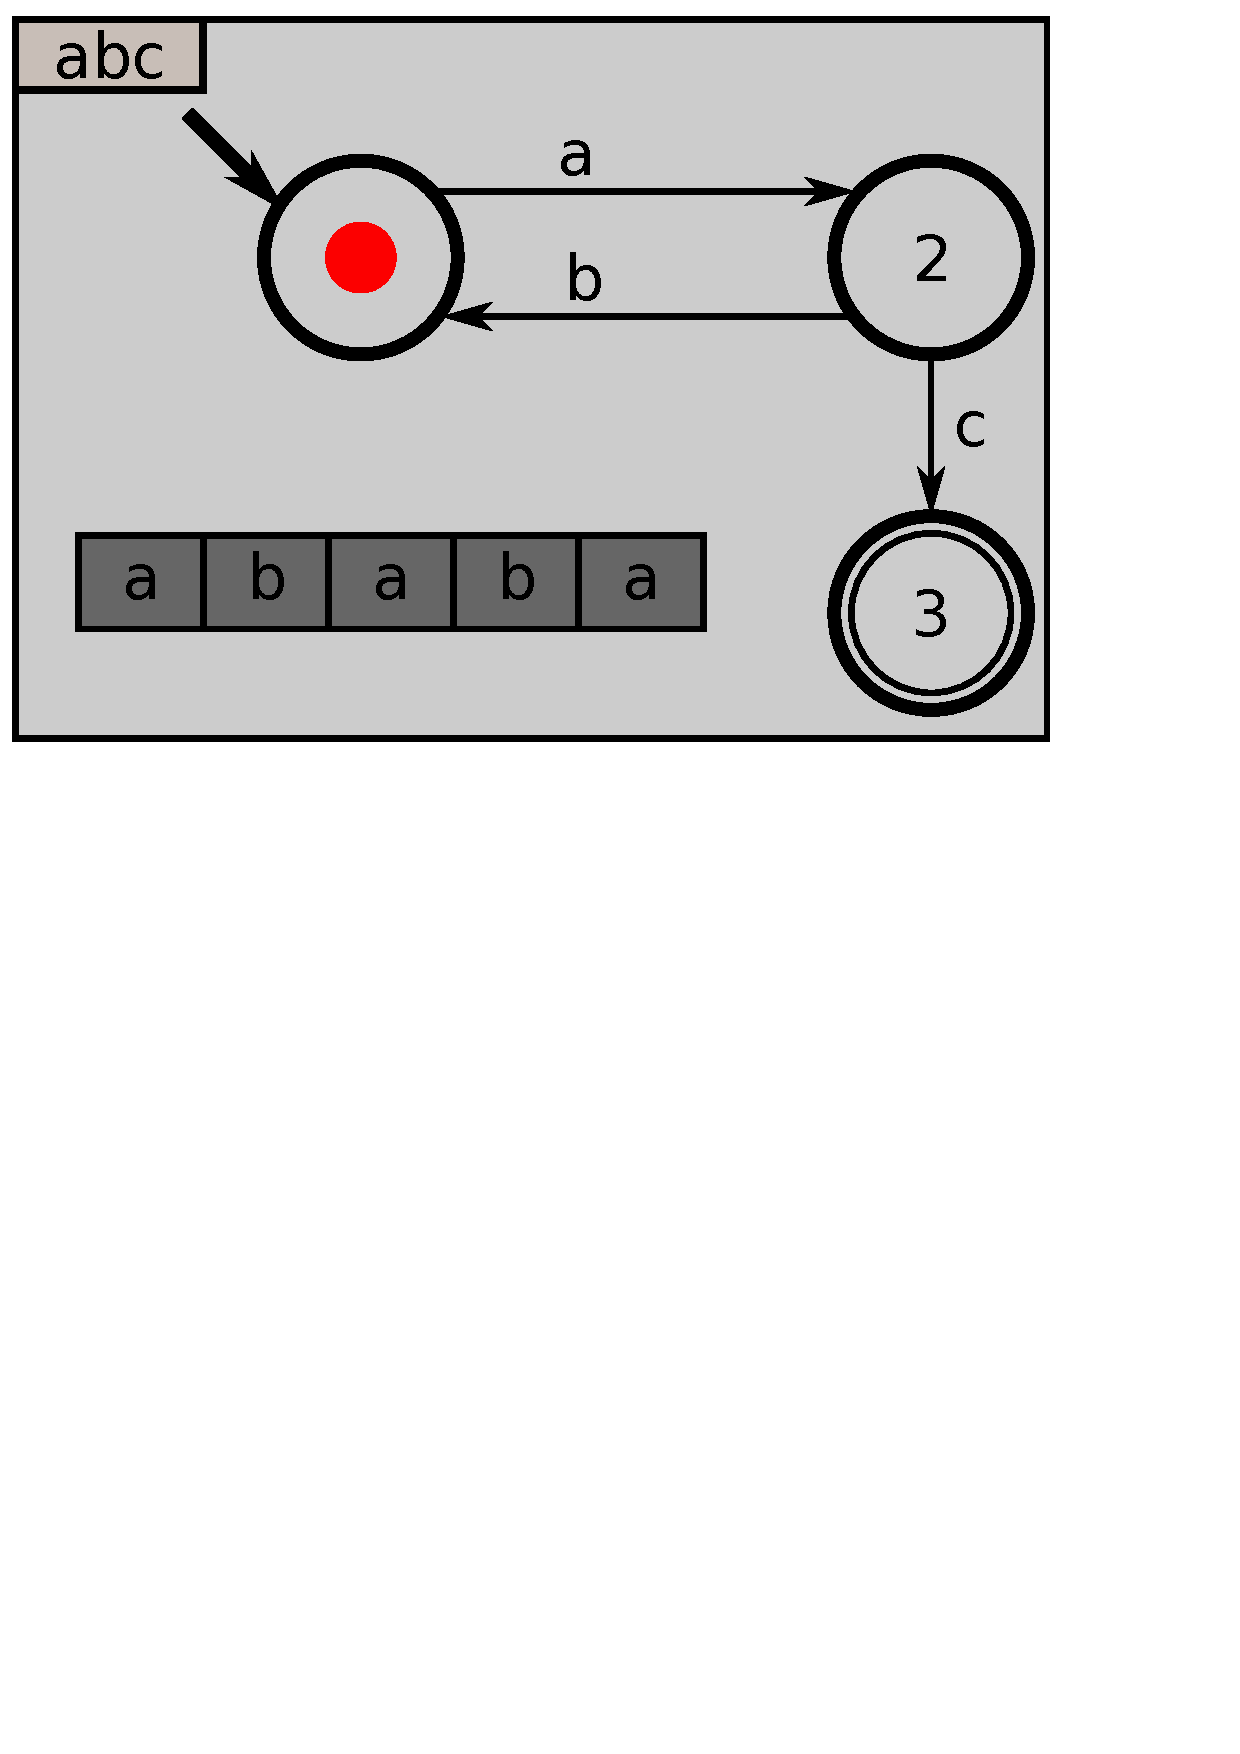
\includegraphics[width=\columnwidth, clip, trim=0cm 17cm 3cm 0cm]{FSM_MX.pdf}%
   \end{subfigure}
  \caption{The \textsf{abc} FSM: a simple model conforming to the specification
   of \autoref{fig:FSM_MM} (left), depicted with the usual concrete syntax, and 
   the starting point of animation of the acceptance of the word 
   $\mathsf{a\cdot b \cdot a \cdot b \cdot a}$ (right)}%
   \label{fig:FSM_M}%
   \Description[A Simple three-States Finite State Machine.]{
   A Simple Finite State Machine, conforming to the specification of the metamodel
   of the previous figure, depicted with the usual concrete syntax (circles for
   \textsf{State}s and arrows for \textsf{Transition}s), that accepts the words
   of the form $\mathsf{a\cdot b \cdot a \cdot b \cdot a}$.
   }
\end{figure}



\autoref{fig:FSM_MM} specifies the metamodel of the Finite State Machine \DSL. 
An \textsf{FSM} is composed of \textsf{State}s identified by a \textsf{name}, and
\textsf{Transition}s that contain a simple \textsf{trigger}. 
\autoref{fig:FSM_M} depicts a simple model consisting of 
three \textsf{State}s and three \textsf{Transition}s, to recognise the regular 
expression $\mathtt{(a\cdot b)^\star\ b}$. 

We assume the classical visual representation for \textsf{FSM}: a \textsf{State}
is represented by a circle labelled with its \textsf{name}; and a 
\textsf{Transition} is represented by an arrow pointing to its \textsf{tgt} and 
labelled by its \textsf{trigger}. We represent the \textsf{current}
\textsf{State} by surimposing a red rounded form (that we call \emph{token}) over
the corresponding \textsf{State} (cf. \autoref{fig:FSM_M}).

\begin{figure}[t]%
   \begin{subfigure}[b]{0.45\columnwidth}
      \centering
      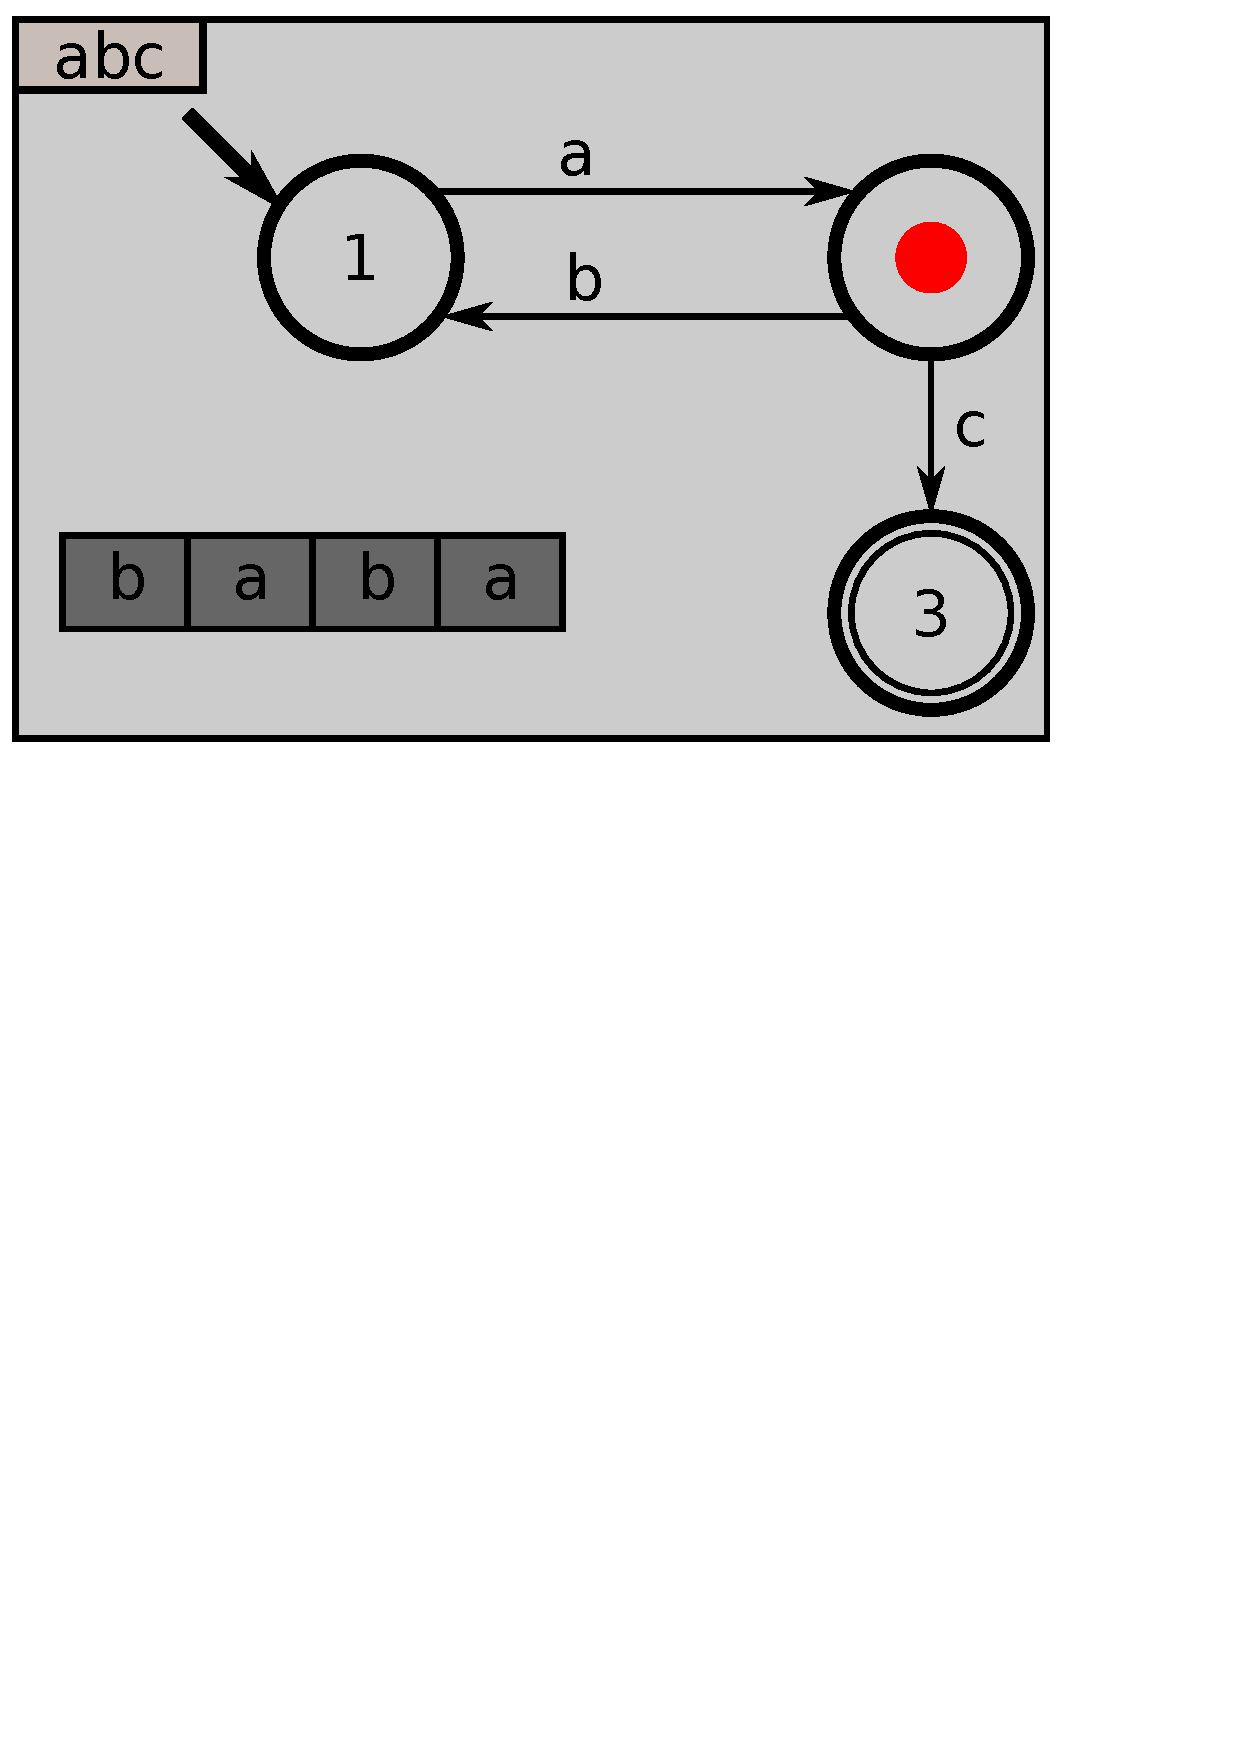
\includegraphics[width=\columnwidth, clip, trim=0cm 17cm 3cm 0cm]{FSM_MA11.pdf}%
      \caption{\emph{FSM.2.1:} Firing \textsf{Transition} \textsf{a} and reaching
      \textsf{State} 2, while consuming the first \textsf{Letter} \textsf{a}.}
      \label{fig:FSM:Model:Animation:FSA1.1}
   \end{subfigure}
   \hfill
   \begin{subfigure}[b]{0.45\columnwidth}
      \centering
      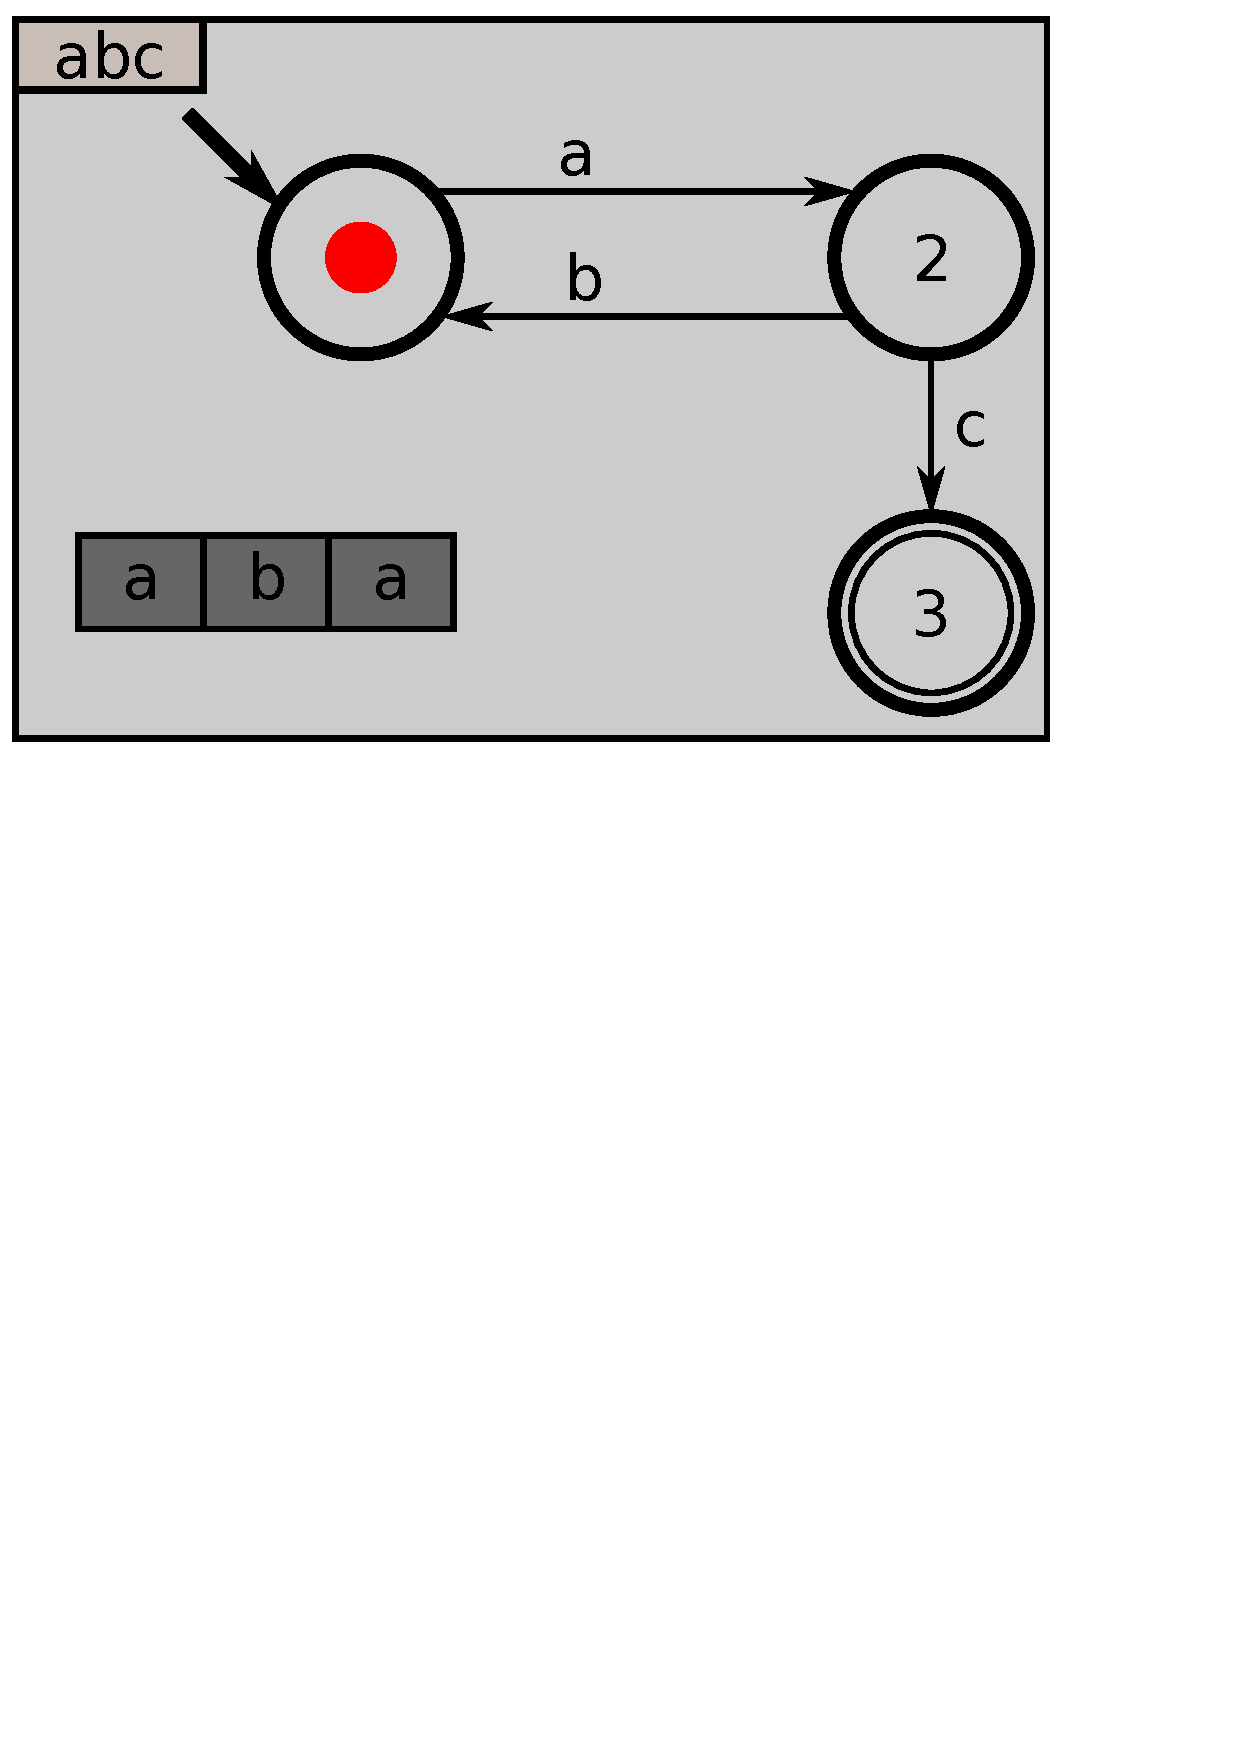
\includegraphics[width=\columnwidth, clip, trim=0cm 17cm 3cm 0cm]{FSM_MA12.pdf}%
      \caption{\emph{FSM.21:} Firing \textsf{Transition} \textsf{b} and reaching
      \textsf{State} 1 again, while consuming \textsf{b}.}
      \label{fig:FSM:Model:Animation:FSA1.2}
    \end{subfigure}
 
    \vskip\baselineskip
    \begin{subfigure}[t]{0.45\columnwidth}
      \centering
      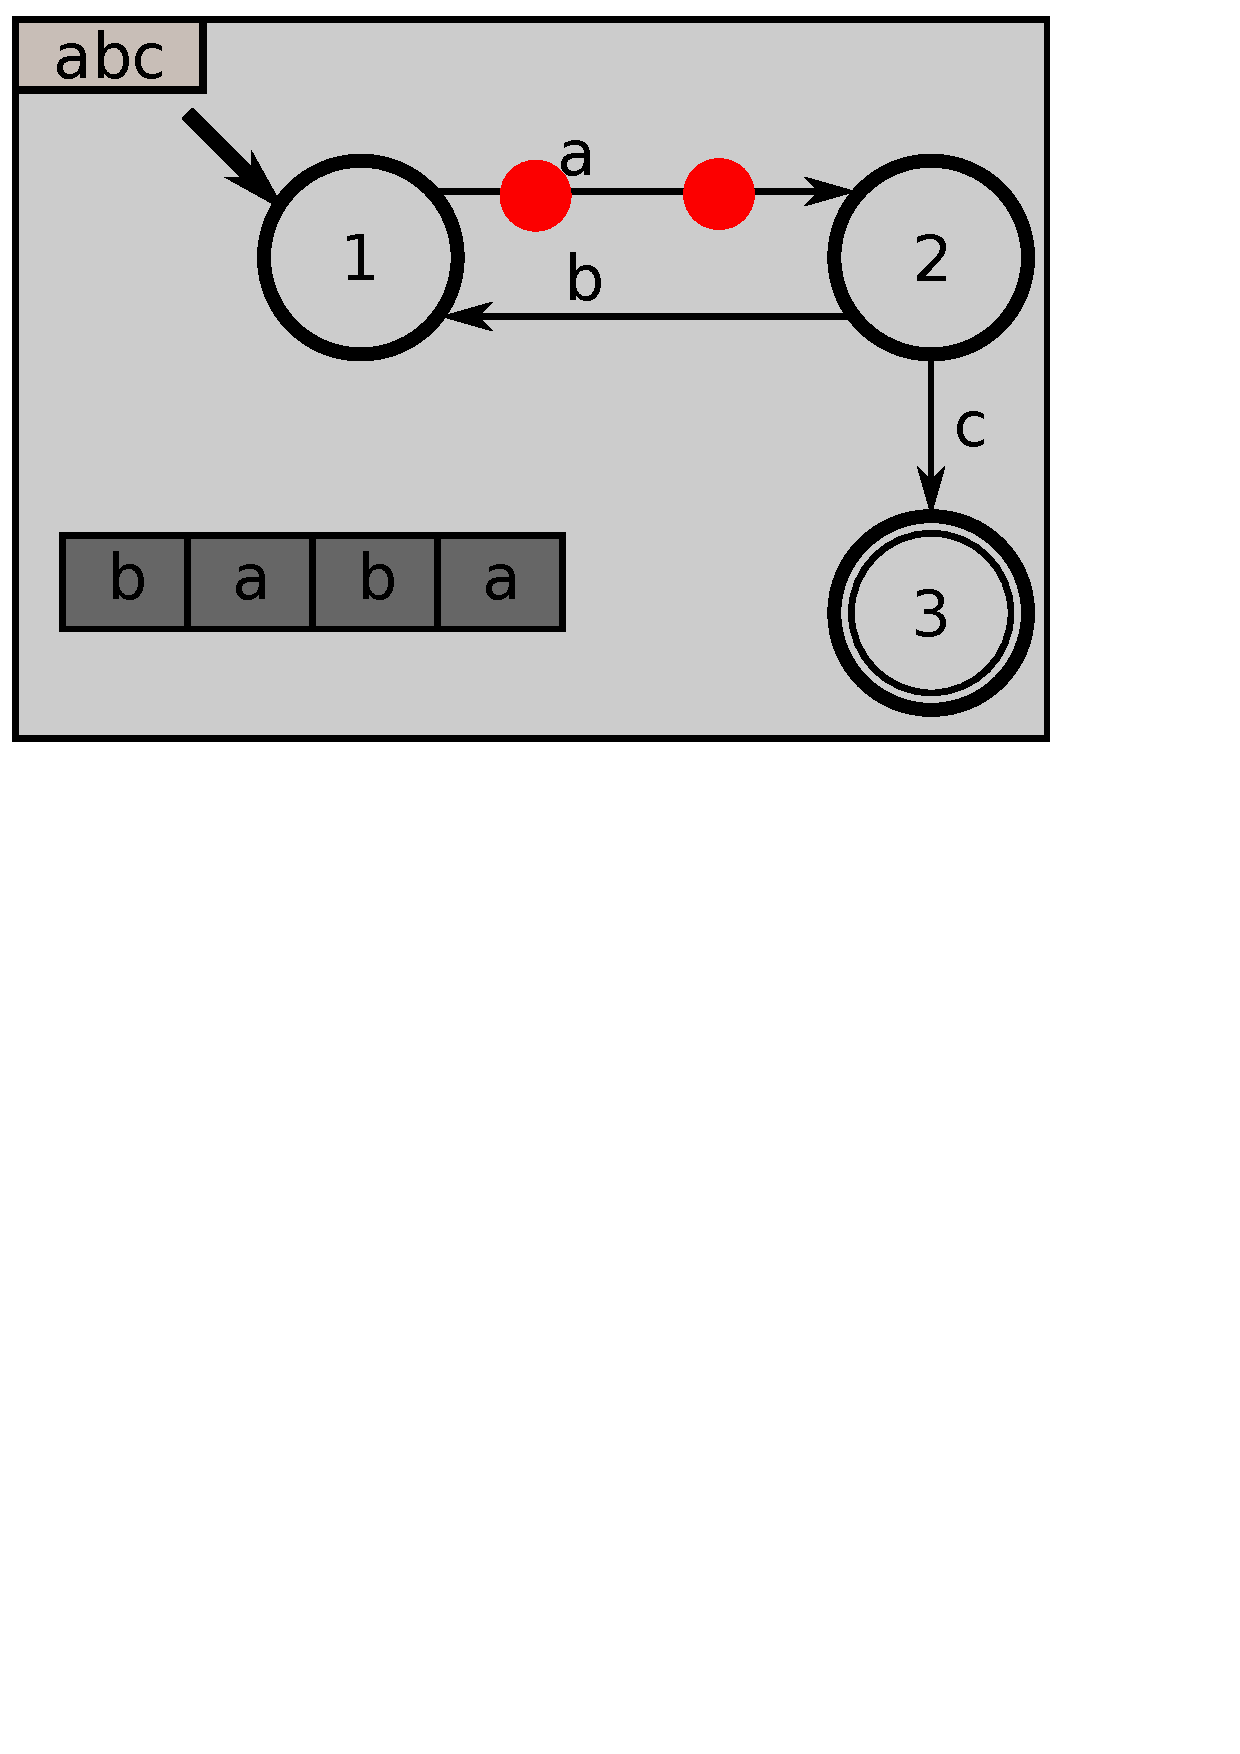
\includegraphics[width=\columnwidth, clip, trim=0cm 17cm 3cm 0cm]{FSM_MA21.pdf}%
      \caption{\emph{FSM.2.2:} First, sliding the \textsf{Token} along the fired
      \textsf{Transition} (with two \textsf{Token} snapshots to reproduce the 
      visual effect).}
      \label{fig:FSM:Model:Animation:FSA2.1}
    \end{subfigure}
    \hfill
    \begin{subfigure}[t]{0.45\columnwidth}
      \centering
      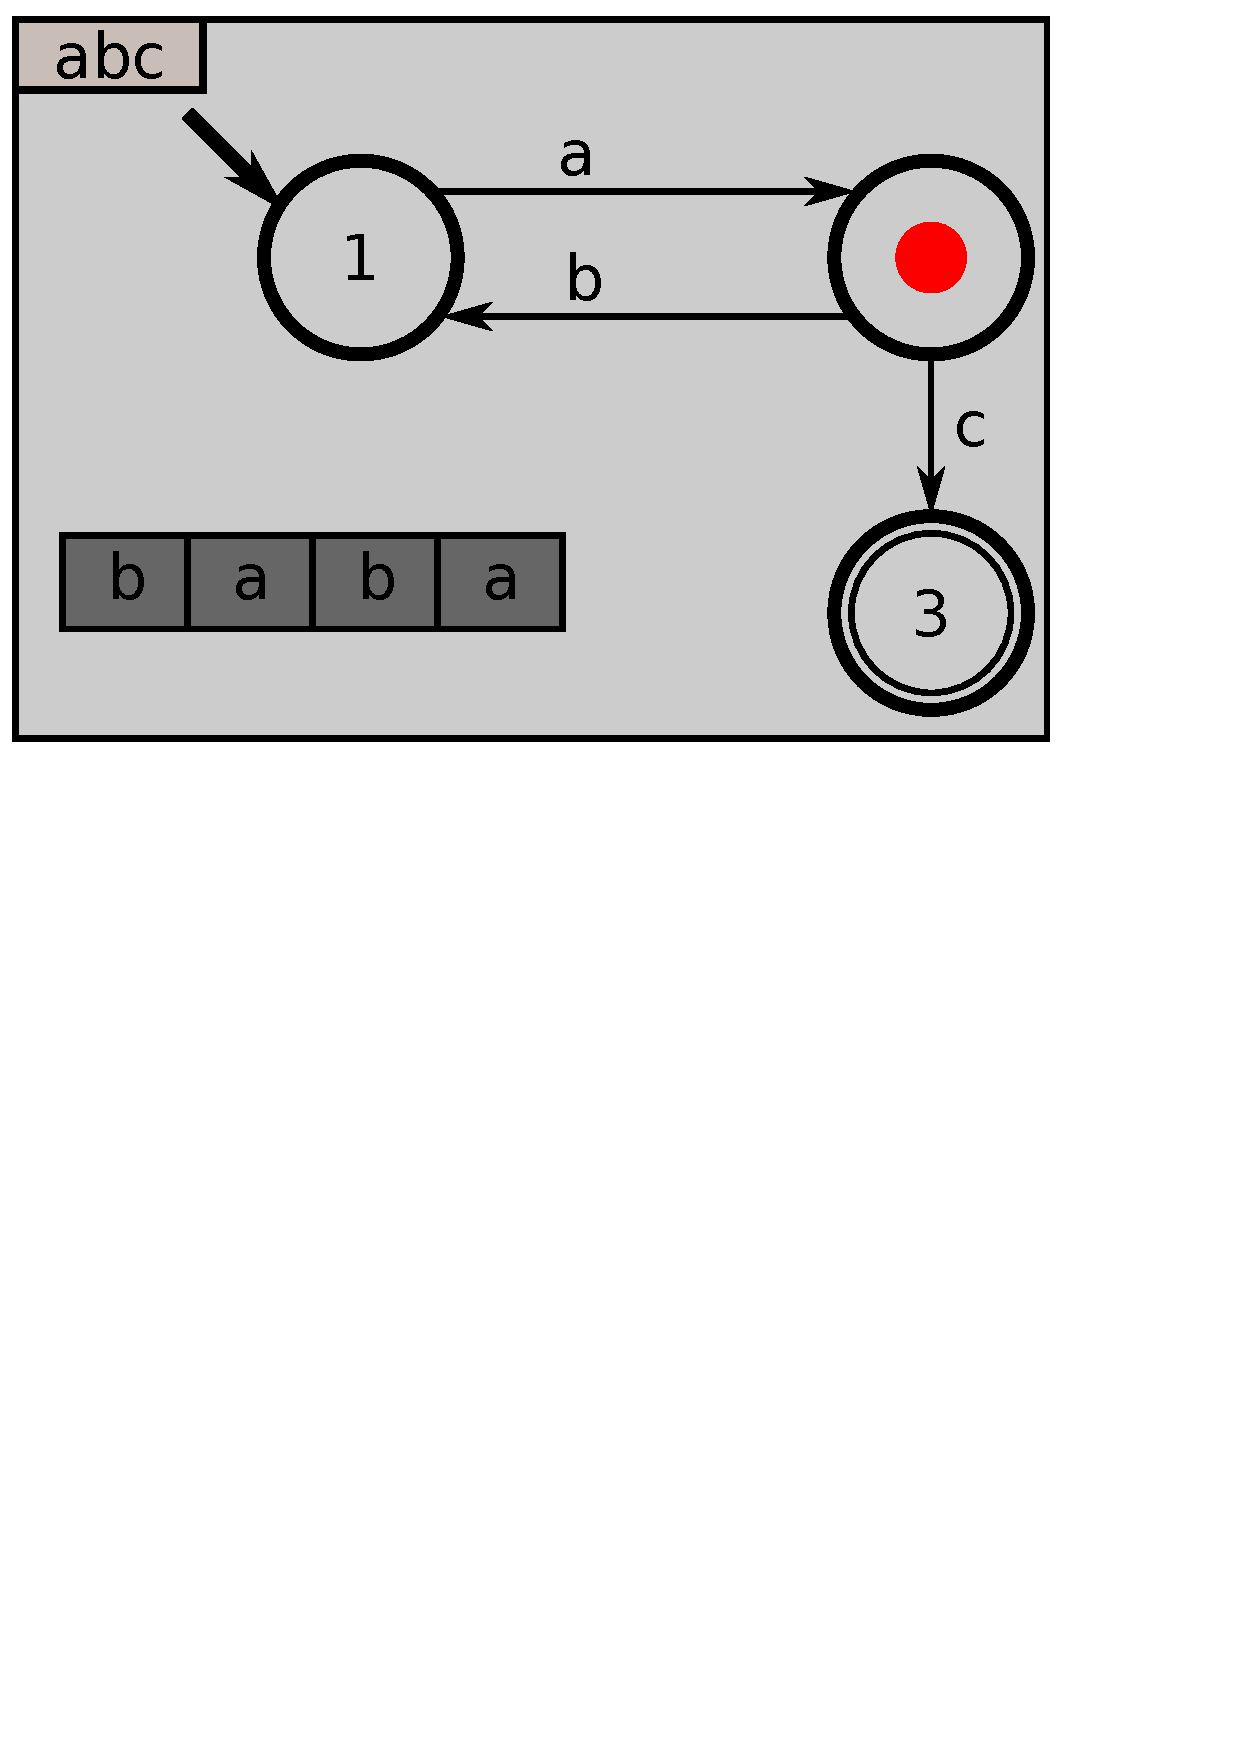
\includegraphics[width=\columnwidth, clip, trim=0cm 17cm 3cm 0cm]{FSM_MA22.pdf}%
      \caption{\emph{FSM.2.2:} Then, moving the \textsf{Token} to the target 
      \textsf{State}}
      \label{fig:FSM:Model:Animation:FSA2.2}
    \end{subfigure}

    \vskip\baselineskip
    \begin{subfigure}[t]{0.45\columnwidth}
      \centering
      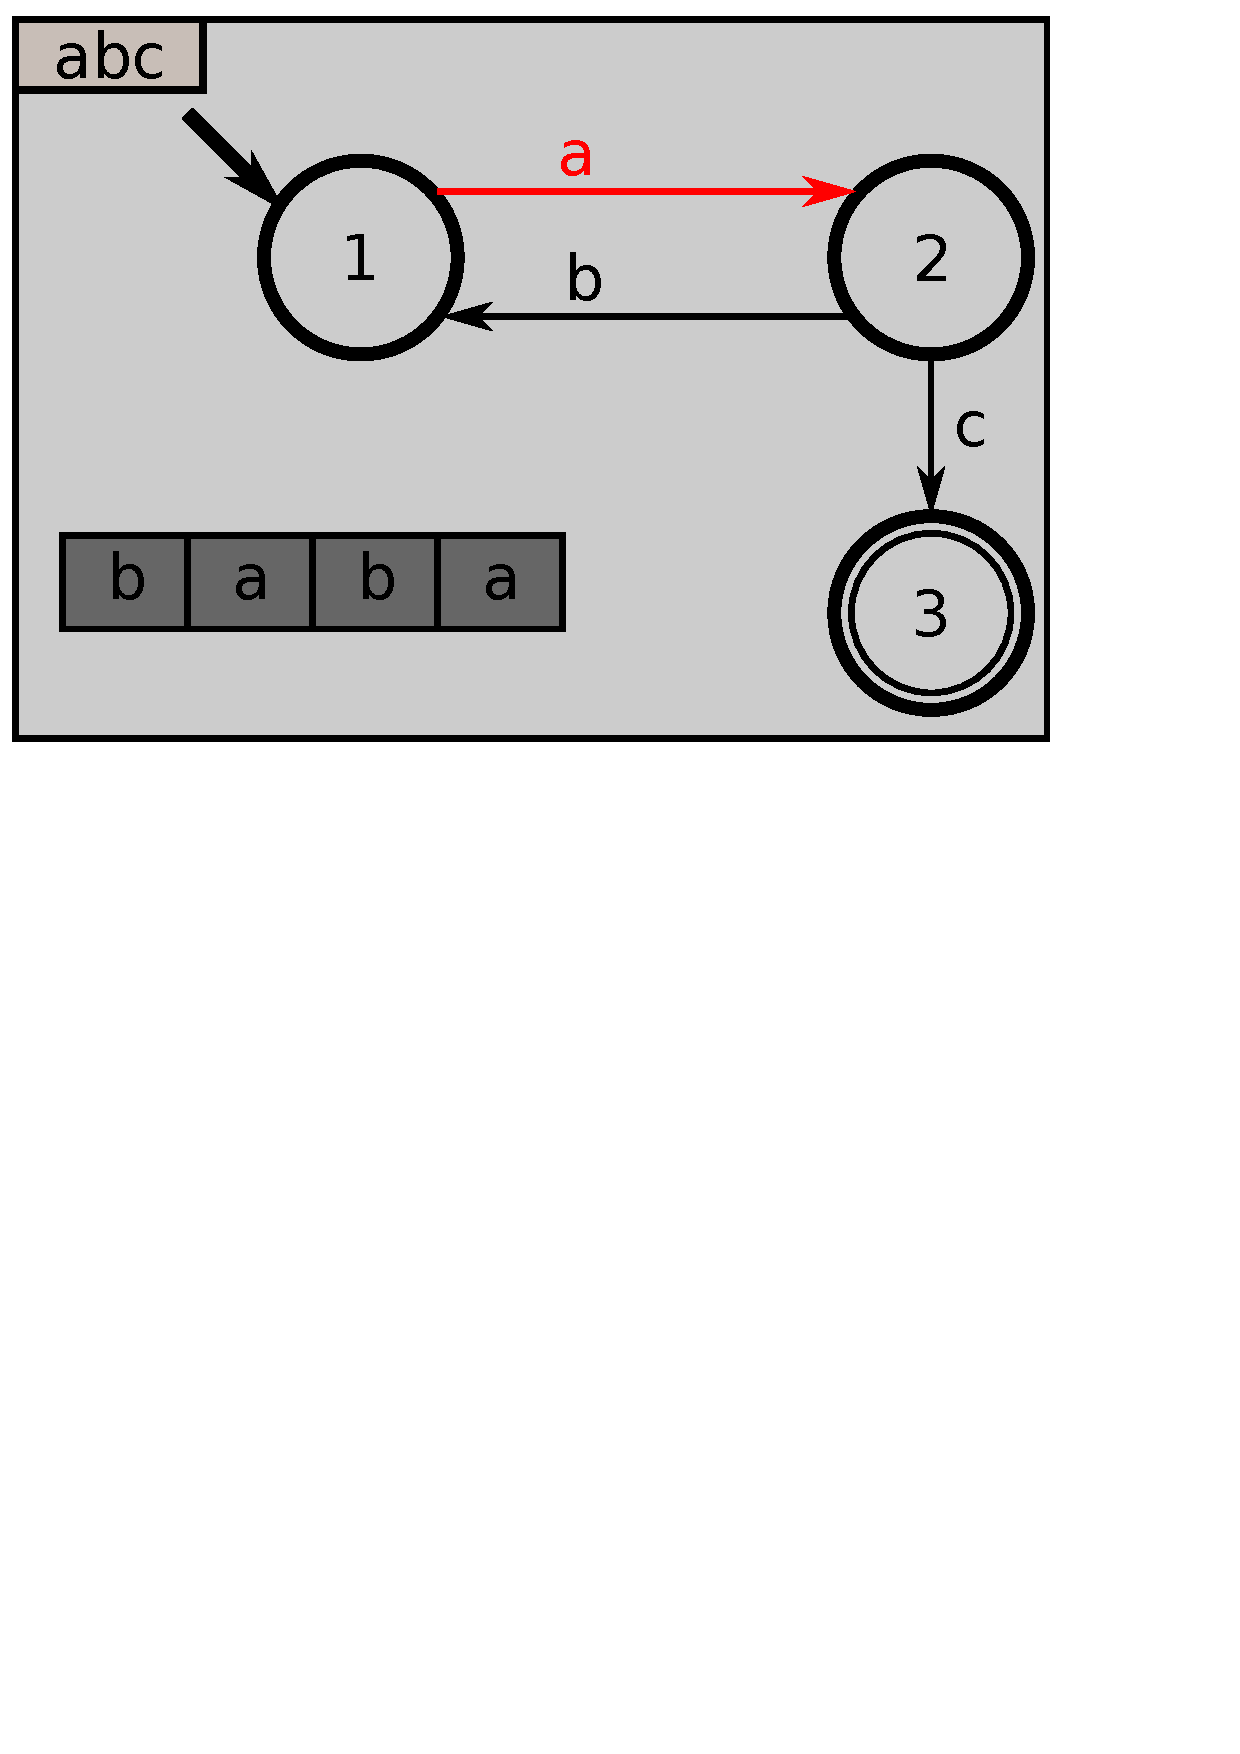
\includegraphics[width=\columnwidth, clip, trim=0cm 17cm 3cm 0cm]{FSM_MA31.pdf}%
      \caption{\emph{FSM.2.3:} First highlighting in red the fired
      \textsf{Transition} (together with its \textsf{trigger}).}
      \label{fig:FSM:Model:Animation:FSA2.3}
    \end{subfigure}
    \hfill
    \begin{subfigure}[t]{0.45\columnwidth}
      \centering
      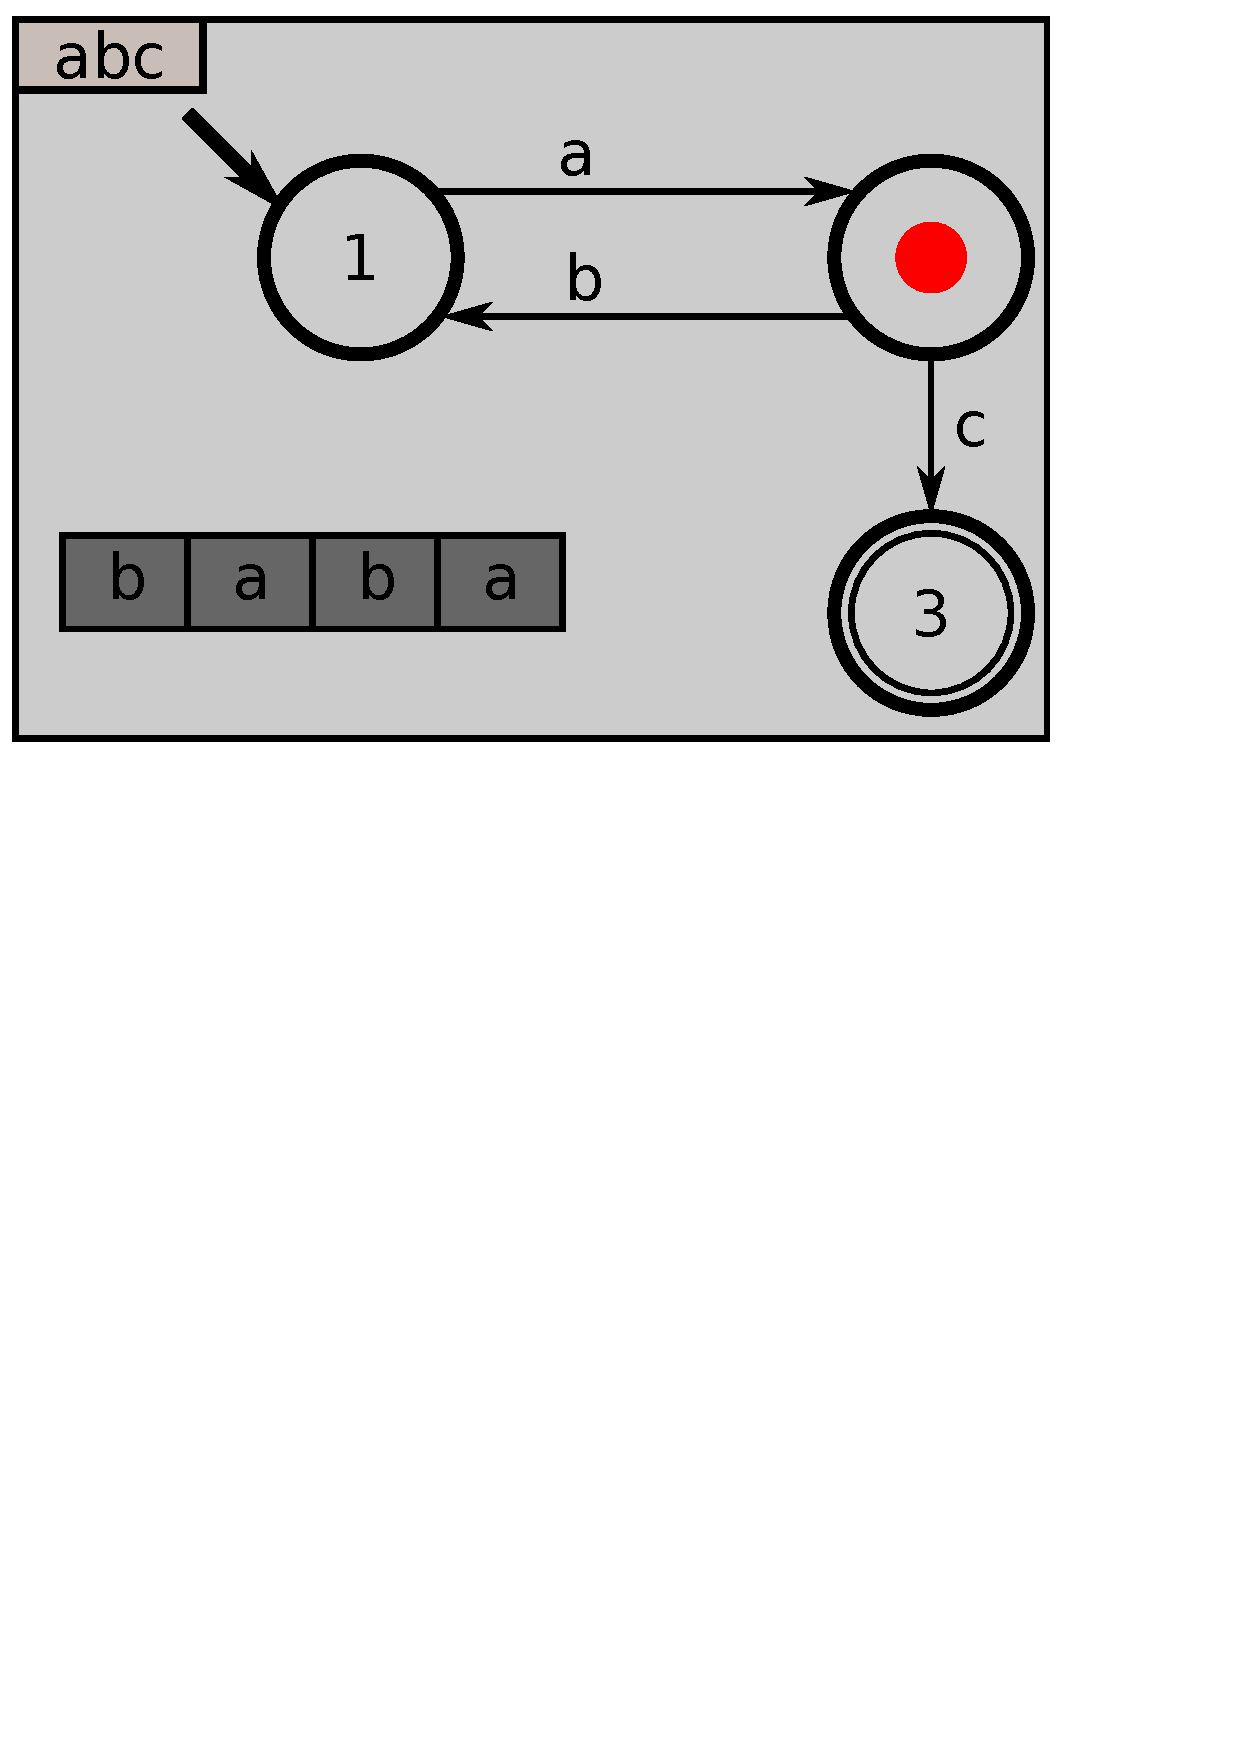
\includegraphics[width=\columnwidth, clip, trim=0cm 17cm 3cm 0cm]{FSM_MA22.pdf}%
      \caption{\emph{FSM.2.3:} Then, moving the \textsf{Token} to the target 
      \textsf{State}}
      \label{fig:FSM:Model:Animation:FSA2.4}
    \end{subfigure}

  \caption{Typical animation steps illustrated: \emph{FSM.2.1} with two acceptance
   steps (top); \emph{FSM.2.2} for sliding along (middle);
   \emph{FSM.2.3} with transition blink (bottom).}%
   \label{fig:FSM_ANIMATION}%
   \Description[Various animations for ]{
   A Simple Finite State Machine, conforming to the specification of the metamodel
   of the previous figure, depicted with the usual concrete syntax (circles for
   \textsf{State}s and arrows for \textsf{Transition}s), that accepts the words
   of the form $\mathsf{a\cdot b \cdot a \cdot b \cdot a}$.
   }
\end{figure}

\subsubsection{Execution}
\label{sec:Examples:FSM:Execution}

The word-accepting semantics is encoded in a transformation called
\textsf{accept} that reads a \textsf{Word} and traverses the \textsf{FSM}. A 
\textsf{Word} is accepted iff the \textsf{State} reached when the \textsf{Word} 
becomes empty is \textsf{FINAL} .

\subsubsection{Animations}
\label{sec:Examples:FSM:Animations}

There are typically two categories of related animations, one for showing the 
progression on the word, the other showing the FSM's current state. 
\begin{description}
   \item[FSM.1] A \textsf{Letter} is consumed from the \textsf{Word} being 
   accepted. This may be performed in two ways:
   \begin{description}
      \item[FSM.1.1] The \textsf{Letter} (and its box) is removed from the \textsf{Word};
      \item[FSM.1.2] The \textsf{Letter} is \st{struck out}, but is present and still readable.
   \end{description}
   \item[FSM.2] A \textsf{Transition} is fired, thus deactivating the current
   \textsf{State} and activating the \textsf{State} the \textsf{Transition} points to.
   This may be realised in different ways:
   \begin{description}
      \item[FSM.2.1] The token disappears from the \textsf{current} \textsf{State}
      and simply reappears inside the updated \textsf{current} \textsf{State}; 
      \item[FSM.2.2] The token disappears from the \textsf{current} \textsf{State},
      and slides along the entire arrow of the fired \textsf{Transition}, then 
      appears in the updated \textsf{current};
      \item[FSM.2.3] The fired \textsf{Transition} blinks in red for 2 seconds,
      then the token disappears from the \textsf{current} \textsf{State},
      before reappearing in the updated \textsf{current}.
   \end{description}
\end{description}
Here again, \textbf{FSM.1} and \textbf{FSM.2} are timely related. 
An MA designer may choose different solutions: a sequential, concurrent (i.e.
indeterministically performing them in an interleaved way), or a precisely timed
approach may suit different needs. Note that the three versions of \textbf{FSM.2}
display different MA \emph{abstraction details} for the same TU, corresponding to
different levels of expertise.

